\section{Premier étude des conditions aux limites transparentes}
\label{sec:TBC}

\subsection{Introduction et quelques exemples de motivation}

\indent Le contenu présenté dans cette section est une introduction aux objectifs qu'on envisage dans ce stage, concernant l'étude des conditions aux limites transparentes (en anglais, \emph{transparent boundary conditions} - TBCs) afin de les appliquer à des méthodes de décomposition de domaine. Cet étude a été développé sur l'équation de KdV, parce que c'était, parmi les modèles étudiés et implémentés jusqu'au moment où on a commencé cette partie du projet, celui pour lequel on a obtenu la meilleure et mas fiable implémentation numérique. En plus, la linéarisation de l'équation de KdV est beaucoup plus évidente que pour les équations de Serre - comme on discutera plus tard, l'étude des TBCs pour des équations linéaires est beaucoup plus développé que pour les non linéaires.

\indent Les TBCs sons construites de façon que la solution calculée dans le domaine comptuationnel fini $\Omega$ coïncide avec la solution du problème dans tout l'espace, restreinte à $\Omega$. En général, ces conditions aux bords son non locales en temps, alors elles doivent être approximés pour permettre une implémentation numérique efficiente \cite{Xavieretal2008}.

%\indent Avant de commencer l'étude de ce sujet pour les modèles de propagation d'ondes, et pour introduire le contenu théorique lié aux TBCs (en suivant  \cite{Japhet2003}), on va présenter et implémenter un example simple, avec de solution y TBCs analytiques connues. On va considérer le problème 1D suivant :

\indent Les TBCs exactes pour le problème

\begin{equation*}
\begin{cases}
\mathcal{A}(u) = f \ \ \text{in} \ \ \Omega\\
u = 0 \ \ \text{on} \ \ \partial\Omega\\
\end{cases}
\end{equation*}

\noindent où $\mathcal{A}$ est un opérateur différentiel partiel, sont données par \cite{Japhet2003}

\begin{equation}
\label{eq:exactTBC}
B_i(u) = \frac{\partial}{\partial n_i}u + D2N(u) = 0
\end{equation}

\noindent où $\partial n_i$ est le vecteur normal sortant à $\Omega_i$ sur $\Gamma$ , et l'opérateur D2N (\emph{Dirichlet to Neumann}) est défini par

$$\left. D2N : \alpha(x) \mapsto \frac{\partial}{\partial n_i^c}v \right\rvert_\Gamma$$

\noindent avec $\alpha$ défini sur $\Gamma$. $v$ est solution du problème suivant,m résolu dans le complémentaire de $\Omega_i$, dénoté $\Omega_i^c$ : 

\begin{equation*}
\begin{cases}
\mathcal{A}(v) = f \ \ \text{in} \ \ \Omega_i^c\\
v = 0 \ \ \text{on} \ \ \partial \Omega_i \backslash \Gamma \\
v = \alpha \ \ \text{on} \ \ \Gamma
\end{cases}
\end{equation*}

\indent Ainsi, on peut interpréter interpréter l'opérateur D2N comme une imposition de continuité de la dérivée de la solution dans la direction normale à l'interface. Par ailleurs, comme son nom indique, cet opérateur construit une dérivée (une condition de Neumann) à partir de la solution dans $\Omega_i^c$ (une condition de Dirichlet).

\indent Présentons d'abord un example simple, avec de solution y TBCs analytiques connues. On va considérer le problème 1D suivant :

\begin{equation*}
\begin{cases}
-u''(x) = 1 \ \ in \ \ \Omega = [0,2]\\
u(0) = 0 \\
u(2) = 0
\end{cases}
\end{equation*}

\noindent dont la solution est

$$u(x) = -\frac{x^2}{2} + x$$

\noindent et, en considérant la partition de $\Omega$ en $\Omega_1 = [0,1]$ et $\Omega_2 = [1,2]$, on va considérer le problème

\begin{equation*}
\begin{cases}
-u_1''(x) = 1 \ \ in \ \ \Omega_1\\
u_1(0) = 0 \\
\mathcal{B}(u_1) = 0 \ \ at \ \ \Gamma=\{1\}
\end{cases}
\end{equation*}

\noindent où la TBC $\mathcal{B}(u)$ est telle que $u|_{\Omega_1} = u_1$.

\indent La fonction $v$, pour la détermination de l'opérateur D2N, est solution de

\begin{equation*}
\begin{cases}
-v''(x) = 1 \ \ in \ \ \Omega_2\\
v(2) = 0 \\
v(1) = \alpha \ \ at \ \ \Gamma=\{1\}
\end{cases}
\end{equation*}

\noindent alors

$$v(x) = -\frac{x^2}{2} + \left(\frac{3}{2} - \alpha \right) + 2\alpha -1$$

\noindent et

$$\left. \frac{\partial}{\partial x}v \right\rvert_{x=1} = \frac{1}{2} - \alpha$$

\indent Finalement, le TBC est

$$B(u_1) = \frac{\partial}{\partial x}u_1 + D2N(u_1) = \frac{\partial}{\partial x}u_1+ \frac{1}{2} - u_1$$

\indent Le problème a été résolu avec une méthode de différences finies, avec des approximations centrées de seconde ordre pour la dérivée spatial, dans deux grilles différentes. La figure \ref{fig:TBClaplace} montre que le TBC construit fournit effectivement une solution convergente à la solution de référence restreinte à $\Omega$.

\begin{center}
	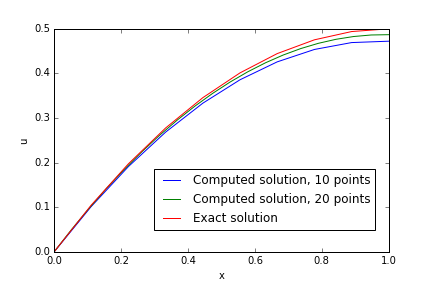
\includegraphics[scale=.5]{figures/TBClaplace.png}
	\captionof{figure}{Solutions pour l'équation de Laplace avec TBC \label{fig:TBClaplace}}
\end{center}

\indent En retournant aux modèles d'ondes, on rappelle que, dans les premières simulations avec les méthodes de \emph{splitting} adoptées pour la résolution de l'équation de KdV, on n'a pas utilisé une application rigoureuse  de conditions aux bords appropriées. En fait, notre objectif principal était de valider la méthode; alors, en imposant des conditions périodiques ou des conditions de Dirichlet ou Neumann homogènes, on a analysé l'évolution de la solution seulement avant son arrivée aux bords.

\indent Avant de commencer l'étude des TBCs pour l'équation de KdV, on va présenter deux examples de motivation à ce travail. Le premier exemple montre très clairement l'influence de conditions aux bords inappropriées sur la solution. On a résolu deux fois le mème problème, avec la même solution initiale, conditions aux bords et discrétisations spatiales et temporales :

\begin{equation*}
    \begin{cases}
    u_t + u_x + (u^2)_x + u_{xxx} = 0 \ , \ \ x \in \Omega=[a,b] \ \ t \in [0, t_{max}] \\
    u(x,0) = \Phi(x) \\
    u(a,t) = 0 \\
    u(b,t) = 0 \\
    u_x(b,t) = 0  \\ 
    \end{cases}
\end{equation*}

\indent La seule différence entre les deux problèmes est la taille de ses domaines: ils ont été choisis de façon que l'onde arrive aux bords (dans le temps de simulation) dans le première problème, mais pas dans le deuxième. La figure \ref{fig:motivational1} montre comme la différence entre les deux solutions augmente avec le temps, en partant du bord et se propageant pour tout le domaine:

\begingroup
	\noindent
	\begin{minipage}[t]{.3\linewidth}
		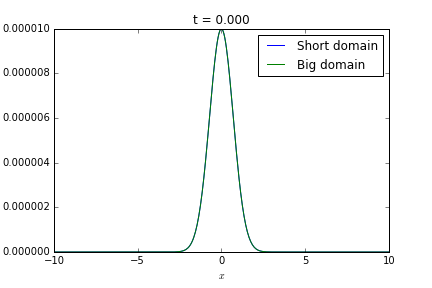
\includegraphics[scale=.3]{figures/motivational1A.png}	
	\end{minipage}
	\hfill
	\begin{minipage}[t]{.3\linewidth}
		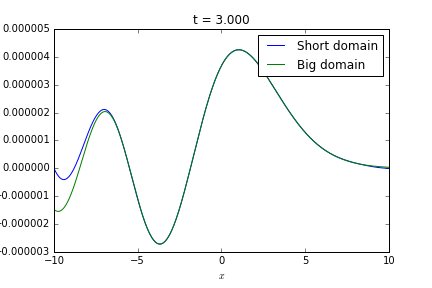
\includegraphics[scale=.3]{figures/motivational1B.png}	
	\end{minipage}
	\hfill
	\begin{minipage}[t]{.3\linewidth}
		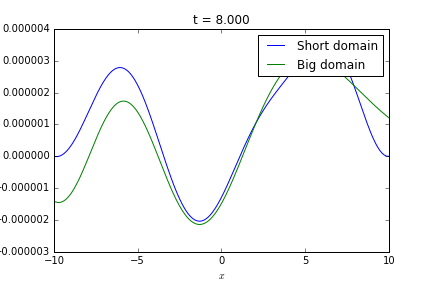
\includegraphics[scale=.3]{figures/motivational1C.png}	
	\end{minipage}
	\captionof{figure}{Premier exemple de motivation : comparaison entre les solutions dans un petit et un large domaines \label{fig:motivational1}}
\endgroup

\indent Alors, on va chercher des conditions aux bords qui puissent bien simuler les TBCs, c'est-à-dire, de façon que la solution calculé dans $\Omega$ soit le même que la solution de tout le domaine restreinte à $\Omega$. Par conséquent, on veut des bords qui n'ont pas d'influence sur la solution, de façon que, quand l'onde arrive au bord, elle puisse simplement "sortir" du domaine.

\indent L'exemple suivant montre une deuxième motivation pour ce travail. On veut résoudre le problème 

\begin{equation*}
    (P_1) \begin{cases}
    u_t + u_x + (u^2)_x + u_{xxx} = 0 \ , \ \ x \in \Omega_1 = [0,L], \ \ t \in [0, t_{max}] \\
    u(x,0) = \Phi(x) \\
    u(0,t) = 0 \\
    u_x(0,t) = 0 \\
    u(L,t) = g(t)  \\ 
    \end{cases}
\end{equation*}

\indent On cherche une fonction  $g(t)$ pour simuler le TBC. Pour atteindre cet objectif, on va d'abord résoudre le problème

\begin{equation*}
    (P_2) \begin{cases}
    u_t + u_x + (u^2)_x + u_{xxx} = 0 \ , \ \ x \in \Omega_2 = [0,2L], \ \ t \in [0, t_{max}] \\
    u(x,0) = \Phi(x) \\
    u(0,t) = 0 \\
    u_x(0,t) = 0 \\
    u(2L,t) = 0  \\ 
    \end{cases}
\end{equation*}

\noindent et on impose $g(t) = u_2(t)$, où $u_2$ est la solution de $(P_2)$. Afin d'obtenir des résultats plus précis, les deux calculs sont réalisés avec les mêmes pas de temps et taille du maillage.

\indent Supposons qu'il y a une unique solution $u_1$ pour $(P_1)$. On peut facilement voir que $u_2|_{\Omega_1}$ est également solution de $(P_1)$. Alors, $u_1 = u_2|_{\Omega_1}$. Ce fait justifie pourquoi notre procédure marche comme une TBC, en fournissant la solution "exacte", comme montre la figure \ref{fig:motivation2}  (détail sur la région proche du bord droit).

\begingroup
\noindent
	\begin{minipage}{.45\linewidth}
		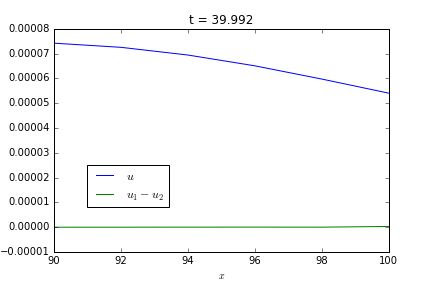
\includegraphics[scale=.5]{figures/motivational2A.png}	
	\end{minipage}
	\hfill
	\begin{minipage}{.45\linewidth}
		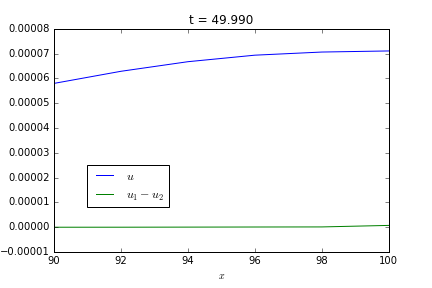
\includegraphics[scale=.5]{figures/motivational2B.png}	
	\end{minipage}
	\captionof{figure}{Deuxième exemple de motivation : solution avec une condition de Dirichlet "exacte" sur le bord à droite \label{fig:motivation2}}
\endgroup

\subsection{Optimisation de conditions aux limites de Robin pour simuler des TBCs}

\indent Malgré le très bon résultat présenté dans le dernier exemple, on ne peut pas appliquer cette procédure en pratique. En fait, calculer la solution dans un domaine plus grand et l'utiliser comme solution exacte pour construire les conditions aux bords n'est qu'une "triche". Alors, on veut plutôt déterminer des approximations pour les TBCs sans avoir une solution de référence.

\subsubsection{Conditions aux limites de Robin jusqu'à la dérivée première}

\indent Dans un approche initial, l'équation de KdV sera résolue dans le domaine $[-L,L]$ avec les conditions aux bords suivants (imposés dans la résolution du deuxième pas de la méthode de \emph{splitting}):

\begin{equation*}
\begin{cases}
    u(-L) = 0 \\
    u_x(-L) = 0 \\
    \alpha u(L) + \beta u_x(L) = 0,  \ \ \alpha,\beta > 0
\end{cases}
\end{equation*}

\indent La troisième condition aux bords consiste en des conditions de Robin, avec des paramètres $\alpha$ et $\beta$ (ou, de façon équivalente, le paramètre  $\beta/\alpha$) qui seront optimisés afin de simuler une TBC sur le bord à droite. Dans un premier moment, on va considérer des conditions de Robin contenant jusqu'à la première dérivée de la solution.

\indent Afin de trouver les coefficients optimaux, on va tester plusieurs paires $(1,\beta/\alpha)$ (y compris les limites $\beta/\alpha \rightarrow 0$ et $\beta/\alpha \rightarrow \infty$, correspondant respectivement aux conditions de Dirichlet et de Neumann) et calculer l'erreur par rapport à la solution de référence $u_{ref}$, calculée dans le domaine $[-2L,2L]$. Deux erreurs seront calculées, pour chaque pas de temps $t_n$ :

\begin{equation*}
e_1^n = \sqrt{\sum_{i=0}^N{\left( u^n_i - (u_{ref})^n_i\right)^2}} 
\end{equation*}

\begin{equation*}
e_2^n =  u^n_N - (u_{ref})^n_N
\end{equation*}

\indent $e_2^n$ est calculé pour montrer que la plus grande partie de l'erreur $e_1^n$ de tout le domaine est due aux bords.
 
\indent Les figures \ref{fig:robin1} à \ref{fig:robinErrorsExample} montrent la solution dans quelques instants et l'évolution de $e_1$ et $e_2$ pour certains valeurs de $\beta/\alpha$. La figure \ref{fig:robinErrorsAll} compare $e_2$  pour plusieurs autres valeurs, y compris le cas de pure Dirichlet  (avec $\alpha = 1, \beta = 0$, alors $log(\beta/\alpha) = -\infty$) et pure Neumann (avec $\alpha = 0, \beta = 1$).

\begingroup
	\noindent
	\begin{minipage}{.45\linewidth}
		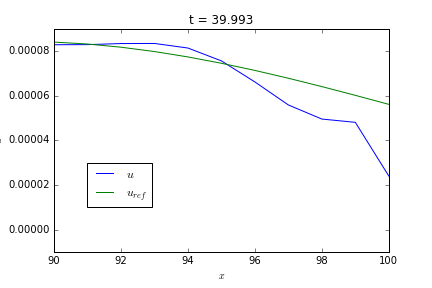
\includegraphics[scale=.5]{figures/robin1A.png}	
	\end{minipage}
	\hfill
	\begin{minipage}{.45\linewidth}
		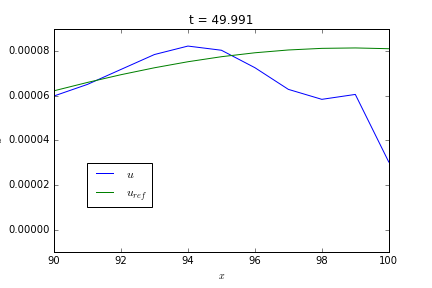
\includegraphics[scale=.5]{figures/robin1B.png}	
	\end{minipage}
	\captionof{figure}{Solution de référence et solution approximée pour  $\beta/\alpha = 1$ \label{fig:robin1}}
\endgroup

\begingroup
\noindent
	\begin{minipage}{.45\textwidth} 
		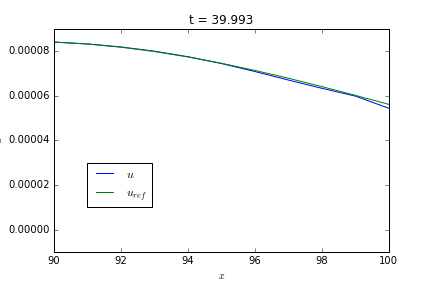
\includegraphics[scale=.5]{figures/robin10A.png}	
	\end{minipage}
	\hfill
	\begin{minipage}{.45\linewidth}
		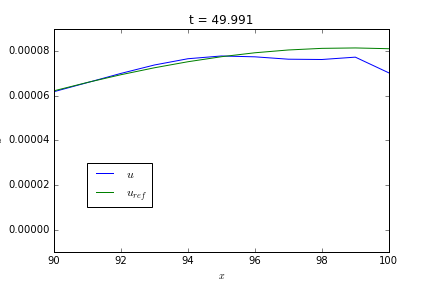
\includegraphics[scale=.5]{figures/robin10B.png}	
	\end{minipage}
	\captionof{figure}{Solution de référence et solution approximée pour  $\beta/\alpha = 10$ \label{fig:robin10}}
\endgroup

\begingroup
\noindent 
	\begin{minipage}{.45\textwidth} 
		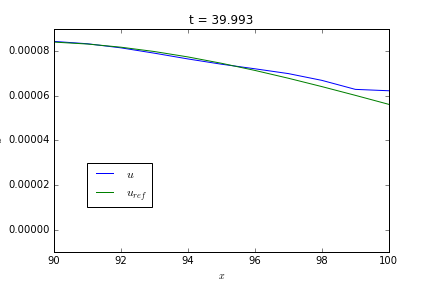
\includegraphics[scale=.5]{figures/robin100A.png}	
	\end{minipage}
	\hfill
	\begin{minipage}{.45\linewidth}
		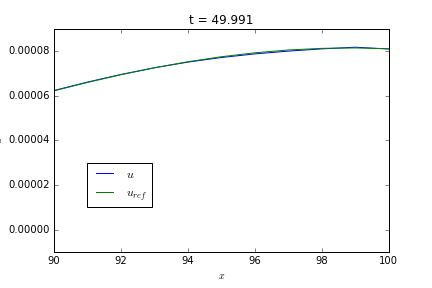
\includegraphics[scale=.5]{figures/robin100B.png}	
	\end{minipage}
	\captionof{figure}{Solution de référence et solution approximée pour  $\beta/\alpha = 100$ \label{fig:robin100}}
\endgroup

\begingroup
\noindent
	\begin{minipage}{.3\textwidth} 
		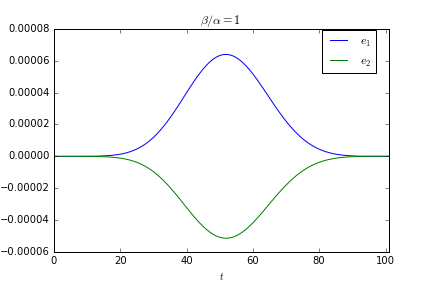
\includegraphics[scale=.3]{figures/robin1Error.png}	
		\captionof{subfigure}{$\beta/\alpha = 1$}
	\end{minipage}
	\hfill
	\begin{minipage}{.3\textwidth} 
		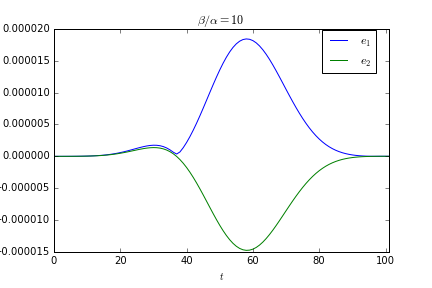
\includegraphics[scale=.3]{figures/robin10Error.png}	
		\captionof{subfigure}{$\beta/\alpha = 10$}
	\end{minipage}
	\hfill
	\begin{minipage}{.3\textwidth}
		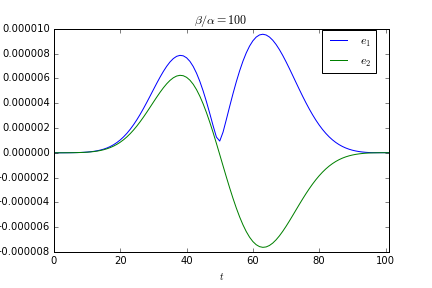
\includegraphics[scale=.3]{figures/robin100Error.png}	
		\captionof{subfigure}{$\beta/\alpha = 100$}
	\end{minipage}
	\captionof{figure}{Erreurs entre la solution approximée et la solution de référence \label{fig:robinErrorsExample}}
\endgroup

\begingroup
\begin{center}
		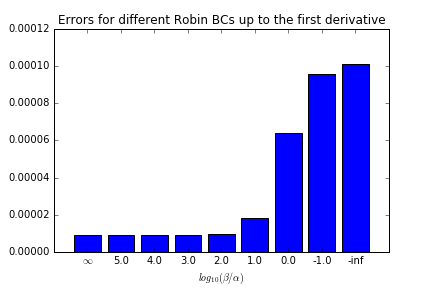
\includegraphics[scale=.6]{figures/robinErrors1.png}
	     \captionof{figure}{Erreur $||e_1| = \sum_{n=0}^{n_{max}}(e^n_1)^2$ entre la solution approximée et la solution de référence pour des plusieurs valeurs de $\beta/\alpha$, avec des conditions aux limits de Robin jusqu'à la dérivée première \label{fig:robinErrorsAll}}
\end{center}
\endgroup

\indent Les résultats présentés dans les figures \ref{fig:robin1} jusqu'à \ref{fig:robinErrorsAll} montrent que des conditions aux bord avec un caractère de Neumann plus fort produisent des meilleures approximations pour le TBC, en comparaison avec des conditions plus proches du pure Dirichlet. Les résultats pour le pure Neumann et pour le Neumann avec un petit mais pas nul Dirichlet terme sont très proches, comme présenté dans le tableau \ref{tab:robinErrorsZoom} pour un étude plus raffiné autour des meilleures valeurs pour $\beta/\alpha$. En fait, imposer la solution nulle aux bord est une condition trop forte, et la condition de Neumann peut capturer de façon plus satisfaisant la lisseté de la solution.

\begingroup
\begin{center}
		\begin{tabular}{c|c}
			$log(\beta/\alpha)$ & Error ($\times 10^{-6}$) \\
			\hline
			2.5 & 8.93\\
			3.0 & 8.87\\
			3.5 & 8.95\\
			4.0 & 8.98\\
			4.5 & 8.99\\
			5.0 & 8.99\\
			$\infty$ & 8.99	
		\end{tabular}
		\captionof{table}{Erreur $||e_1| = \sum_{n=0}^{n_{max}}(e^n_1)^2$ pour quelques valeurs de $\beta/\alpha$ autour des meilleurs résultats \label{tab:robinErrorsZoom}}
\end{center}
\endgroup

\subsubsection{Conditions aux limites de Robin jusqu'à la dérivée seconde}

\indent On a répété les tests décrits ci-dessus, mais en remplaçant les conditions au bord droit par $\alpha u(L) + \beta u_x(L) + \gamma u_{xx}(L) = 0,  \ \ \alpha,\beta, \gamma > 0$.

\indent Les valeurs de $\alpha$ et $\beta$ sont fixés et égaux à celui qui a donné l'erreur minimal dans les simulations précédents ($(\alpha,\beta) = (1,1000)$). On montre directement le graphe contenant les erreurs pour des plusieurs valeurs de $\gamma/\beta$ (figure \ref{fig:robinErrorsAll2}). De façon similaire aux conclusions faites ci-dessus, on a observé une meilleure approximation du TBC pour des valeurs plus fortes de $\gamma/\beta$ (étant l'erreur presque constant à partir d'un certain seuil, comme montre le tableau \ref{tab:robinErrors2Zoom}). En fait, même l'erreur le plus grande dans la figure \ref{fig:robinErrorsAll2} ($||e_1|(\gamma/\beta = 0.01) = 8.78 \times 10^{-6}$) est plus petit que le meilleur cas présenté dans le tableau \ref{tab:robinErrorsZoom}.

\begingroup
\begin{center}
		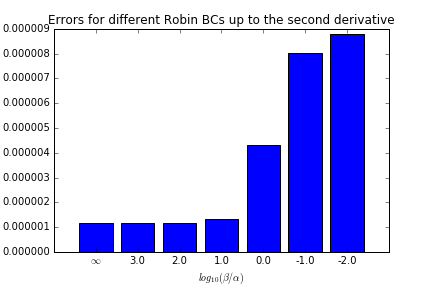
\includegraphics[scale=.6]{figures/robinErrors2.png}
	     \captionof{figure}{Erreur $||e_1| = \sum_{n=0}^{n_{max}}(e^n_1)^2$ entre la solution approximée et la solution de réference pour des plusieurs valeurs de $\gamma/\beta$, avec des conditions aux limits de Robin jusqu'à la dérivée seconde  \label{fig:robinErrorsAll2}}
\end{center}
\endgroup

\begingroup
\begin{center}
		\begin{tabular}{c|c}
			$log(\gamma/\beta)$ & Error ($\times 10^{-6}$) \\
			\hline
			2.0 & 1.157665\\
			2.5 & 1.157382\\
			3.0 & 1.157280\\
			3.5 & 1.157247\\
			4.0 & 1.157236\\
			4.5 & 1.157233\\
			$\infty$ & 1.157231	
		\end{tabular}
		\captionof{table}{Error $||e_1| = \sum_{n=0}^{n_{max}}(e^n_1)^2$ for some values of $\gamma/beta$ around the best ones \label{tab:robinErrors2Zoom}}
\end{center}
\endgroup

\subsubsection{Conclusion partiale} 

\indent Pour résumer cet étude initial des conditions transparentes, on a cherché à les approximer par des conditions aux bords de Robin, écrites en fonction de coefficients ajustables afin d'attribuer différentes importances à chacun des termes (la solution et ses dérivées). L'idée était de tester plusieurs combinaisons de ces coefficients afin de les optimiser (au sens de minimiser l'erreur entre la solution calculée dans $[-L,L]$ et la solution de référence, calculée dans $[-2L,2L]$) . Comme on a décrit ci-dessus, les conditions de Robin qui prennent en compte la continuité de la solution testée (i.e., avec des coefficients plus grands pour les termes des dérivées) ont produit des meilleurs résultats. Alors, la TBC basée sur la première dérivée a été plus efficiente que celle basée seulement sur la solution; et la TBC basée sur la seconde dérivée a été encore meilleure. Finalement, on a observé que l'amélioration de la solution est négligeable au-dessus une certaine relation entre les coefficients.

























\section{Conditions aux limites transparentes approximées pour l'équation de dispersion}

\indent Dans  \cite{besse2015}, des conditions aux limites transparents exactes sont dérivées pour l'équation de KdV linéarisée (ou équation de Airy) :

\begin{equation}
 	\label{eq:LKdV}
 	u_t + U_1u_x + U_2u_{xxx} = h(t,x), \ \ t \in \mathbb{R}^+, \ \ x \in \mathbb{R}
\end{equation}

\noindent où $U_1 \in \mathbb{R}$, $U_2 \in \mathbb{R}^+_*$ et $h$ est un terme de source.

\indent Pour le problème homogène à valeur initiale

\begin{equation*}
\begin{cases}
	u_t + U_1u_x + U_2u_{xxx} = h(t,x), \ \ t \in \mathbb{R}^+, \ \ x \in [a,b] \\
	u(0,x) = u_0(x), \ \ x \in [a,b] \\
	+ \text{boundary conditions} \nonumber
\end{cases}
\end{equation*}

\noindent les TBCs sont données \cite[équations 2.17,2.18]{besse2015} par 

\begin{equation}
\label{eq:continuousTBC}
\begin{gathered}
        u(t,a) - U_2 \laplinv \left( \frac{\lambda_1(s)^2}{s} \right) * u_x(t,a) - U_2 \laplinv \left( \frac{\lambda_1(s)}{s} \right) * u_{xx}(t,a) = 0 \\ 
        u(t,b) - \laplinv \left( \frac{1}{\lambda_1(s)^2} \right) * u_{xx}(t,b) = 0 \\
        u_x(t,b) - \laplinv \left( \frac{1}{\lambda_1(s)} \right) * u_{xx}(t,b) = 0 
\end{gathered}
\end{equation}

\noindent où $\laplinv$ dénote la transformée inverse de Laplace, $s \in \mathbb{C},\ Re(s)>0$ est la fréquence de Laplace et $\lambda_1$ est, parmi les trois racines du polynôme caractéristique cubique obtenu en résolvant \eqref{eq:LKdV} dans l'espace de Laplace, la seule avec partie réelle négative. \cite{zheng2008}

\indent On va concentrer nos efforts dans le cas $U_1 = 0, U_2 = 1$, qui fournit l'équation de KdV linéarisée avec seulement la partie dispersive (qu'on appellera \emph{équation de dispersion}) :

\begin{equation}
	\label{eq:DKdV}
	u_t + u_{xxx} = 0
\end{equation}

\indent Dans ce cas, aussi d'après \cite{zheng2008}, la seule racine avec partie réelle négative est

\begin{equation}
	\label{eq:lambda}
			\lambda(s) = \lambda_1(s) =  -\sqrt[3]{s} 
\end{equation}

\indent Cependant, le calcul des TBCs \eqref{eq:continuousTBC} n'est pas simple en raison de la transformée inverse de Laplace, qui donnent à ces conditions un caractère nonlocal en temps. Ainsi, on va proposer des approximations pour la racine \eqref{eq:lambda} qui évitent les intégrations en temps, en générant des TBC considérablement plus simples.

\indent Évidemment, comme on va à vérifier dans les résultats présentés dans cette section, les TBCs approximées ne sont pas si précises comme les TBCs proposées par \cite{besse2015} (qui les dérive pour la version discrète de l'équation de KdV linéarisée). Néanmoins, nos objectifs sont très différents de ceux de \cite{besse2015} : tandis qu'ils cherchent à minimiser l'erreur de la solution calculée (comparée avec la solution analytique) due aux conditions aux bords, on cherche ici à utiliser les TBCs approximées comme conditions aux limites à l'interface (IBCs), dans le contexte d'une Méthode de Décomposition de Domaine (DDM). Ainsi, notre objectif s'appuie sur la convergence de la solution fournie par la DDM à la solution du même problème résolu dans le monodomain,  indépendamment des erreurs dans les bords extérieurs. 

\indent Pour dériver nos approximations, on rappele les propriétés suivantes \cite{laplaceTransform} de la transformée de Laplace:

\begin{itemize}
	\item Linearity :
		\begin{equation}
			\label{eq:linearityLaplace}
				\laplinv \left[a_1\hat{u}_1(s,x) + a_2\hat{u}_2(s,x)\right] = a_1u_1(t,x) + a_2u_2(t,x)
		\end{equation}
	\item First Derivative : 
		\begin{equation}
			\label{eq:firstDerivativeLaplace}
			\laplinv \left[ s\hat{u}(s,x) \right] = u_t(t,x) + \laplinv \left[ u(0,x) \right] =  u_t(s,t) +  u(0,x) \delta (t)
		\end{equation}
	\item Second Derivative : 
		\begin{equation}
			\label{eq:secondDerivativeLaplace}
			\begin{aligned}
			\laplinv \left[ s^2\hat{u}(s,x) \right] = & u_{tt}(t,x) + \laplinv \left[ su(0,x) + u_{t}(0,x)\right] = \\
																		   & u_{tt}(s,t) + u(0,x)\delta_t(t) +  u_t(0,x)\delta (t)
			\end{aligned}
		\end{equation}
	\item Convolution :
	\begin{equation}
		\label{eq:convolutionLaplace}
		\laplinv \left[ \hat{u}_1(s,x)\hat{u}_2(s,x)\right] = \laplinv \left[ \hat{u}_1(s,x)\right] * \laplinv \left[ \hat{u}_2(s,x)\right]
	\end{equation}
\end{itemize} 

\noindent où $\delta (t)$ est la fonction delta de Dirac et $*$ note l'opérateur de convolution.

\indent Les propriétés \eqref{eq:linearityLaplace} jusqu'à \eqref{eq:convolutionLaplace} nous motivent à approximer les opérandes des transformées inverses de Laplace dans \eqref{eq:continuousTBC} par des polynômes dans $s$. On va implémenter et tester des approximations avec des polynômes constants et des polynômes linéaires :

\subsection{Approximation des TBCs utilisant des polynômes constants}

\indent On va utiliser le polynôme constant $P_0(s) = c$  pour approximer $\frac{\lambda^2}{s}$. Par ailleurs, en raison de \eqref{eq:lambda}, on peut approximer les autres opérandes des transformées inverses de Laplace dans \eqref{eq:continuousTBC} uniquement en fonction de $c$ :

\begin{equation}
	\label{eq:appP0}
	\frac{\lambda^2}{s}  = c, \qquad
	\frac{\lambda}{s}  = -c^2, \qquad
	\frac{1}{\lambda_1(s)^2}  = c^2,\qquad 
	 \frac{1}{\lambda_1(s)}  = -c 
\end{equation}

\indent En remplaçant \eqref{eq:appP0}  dans \eqref{eq:continuousTBC} et en considérant des approximations différentes pour les bords à gauche et à droite (respectivement avec les coefficients $c_L$ et $c_R$), on obtient les TBC approximées :

\begin{equation}
\label{eq:appTBCP0}
    \begin{gathered}
        \Theta_1^{c_L}(u,x) = u(t,x) - c_L u_x(t,x)  + c_L^2  u_{xx}(t,x) = 0 \\
        \Theta_2^{c_R}(u,x) = u(t,x) - c_R^2  u_{xx}(t,x) = 0 \\
        \Theta_3^{c_R}(u,x) = u_x(t,x) + c_R u_{xx}(t,x)= 0 
    \end{gathered}
\end{equation}

\indent En considérant un domaine discret avec une taille de maille $\Delta x$ et des points $x_0, ..., x_N$ , et en utilisant des approximations par différences finies, les TBC approximées \eqref{eq:appTBCP0} sont discrétisées comme

\begin{equation}
\label{eq:appDiscTBCP0}
    \begin{gathered}
        u_0 - c_L \frac{u_1 - u_0}{\Delta x}  + c_L^2  \frac{u_0 -2u_1 + u_2}{\Delta x^2} = 0 \\
        u_N - c_R^2    \frac{u_N -2u_{N-1} + u_{N-2}}{\Delta x^2} = 0 \\
        \frac{u_N - u_{N-1}}{\Delta x}  + c_R^2    \frac{u_N -2u_{N-1} + u_{N-2}}{\Delta x^2} = 0 
    \end{gathered}
\end{equation}

\subsubsection{Tests de validation de l'approximation}

\indent Afin de valider nos approximations, observer son comportement général quand on fait varier les coefficients $c_L$ et $c_R$, et comparer nos résultats avec ceux obtenus par \cite{zheng2008} et \cite{besse2015} , on va résoudre le même test numérique considéré dans ces papiers : 

\begin{subnumcases}{}
\label{eq:testCaseBesse1}
 u_t + u_{xxx} = 0, \ \ x \in \mathbb{R} \\
 \label{eq:testCaseBesse2}
 u(0,x) = e^{-x^2}, \ \ x \in \mathbb{R}  \\
 \label{eq:testCaseBesse3}
 u \rightarrow 0, \ \ |x| \rightarrow \infty
\end{subnumcases}

\indent La solution fondamentale de \eqref{eq:testCaseBesse1} et la solution exacte du problème  \eqref{eq:testCaseBesse1} - \eqref{eq:testCaseBesse3} sont donnés, respectivement, par

\begin{equation}
    E(t,x) = \frac{1}{\sqrt[3]{3t}}Ai\left(\frac{x}{\sqrt[3]{3t}} \right)
\end{equation}

\begin{equation}
	\label{eq:exactSolution}
    u_{exact}(t,x) = E(t,x) * e^{-x^2}
\end{equation}

\noindent où $Ai$ est la fonction d'Airy.

\indent En suivant \cite{zheng2008} et \cite{besse2015}, le problème sera résolu dans le domaine spatiale $[-6,-6]$, pour $0 \leq t \leq T_{max}$, avec $T_{max} = 4$. La taille de maille est $\Delta x = 12/500 = 0.024$ et, aussi comme fait \cite{besse2015}, le pas de temps est $\Delta t = 4/2560 = 0.0015625$.

\indent Pour une évaluation quantitative des résultats, on calculera les mêmes erreurs définies par \cite{besse2015}: pour chaque instant $t_n = n\Delta t$, on définit l'erreur $l^2-$ relative

$$e^n = \frac{\left\Vert u_{exact}^n - u_{computed}^n\right\Vert_2}{\left\Vert u_{exact}^n\right\Vert_2}$$

\noindent et, dans tout l'intervalle de temps, l'erreur maximale $e^n$ et la norme $l^2$ de $e^n$, données respectivement par

\begin{equation}
 e_{Tm} = \max\limits_{0 < n < T_{max}} (e^n), \qquad
    e_{L2} = \sqrt{ \Delta t \sum_{n=1}^{T_{max}} (e^n)^2 }
\end{equation}

\indent Afin de vérifier l'influence de $c_L$ et $c_R$ sur les solutions calculées (et, possiblement, identifier des intervalles de valeurs qui donnent les meilleures approximations pour les TBCs), on a fait des tests avec tous les paires possibles $(c_L,c_R) \in \{-10,-1,-0.1,0,0.1,1,10\}^2$. Les résultats ont été classifiées selon leurs erreurs $e_{L2}$ (un critère basé sur l'erreur $e_{Tm}$ fournit un résultat similaire). La figure \ref{fig:firstTestsP0} montre, pour quelques instants, une comparaison entre la solution exacte, la meilleure et la pire. Pour nommer la pire solution, on n'a pas considéré les solutions divergentes (selon le critère arbitraire $e_{L2} > 10$).

\begingroup
\begin{minipage}{.5\linewidth}
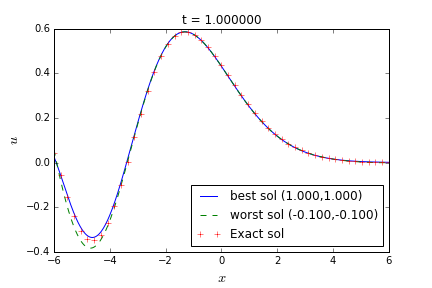
\includegraphics[scale=.5]{figures/BessefirstTestsP0Snap2.png}
\end{minipage}
\begin{minipage}{.5\linewidth}
	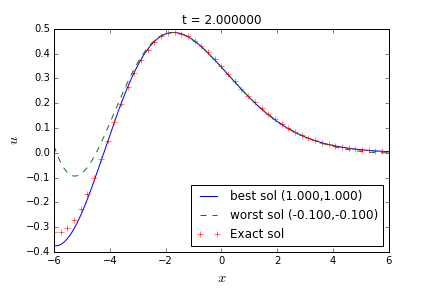
\includegraphics[scale=.5]{figures/BessefirstTestsP0Snap3.png}
\end{minipage}
\begin{minipage}{.5\linewidth}
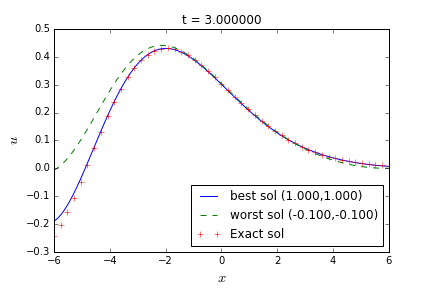
\includegraphics[scale=.5]{figures/BessefirstTestsP0Snap4.png}
\end{minipage}
\begin{minipage}{.5\linewidth}
	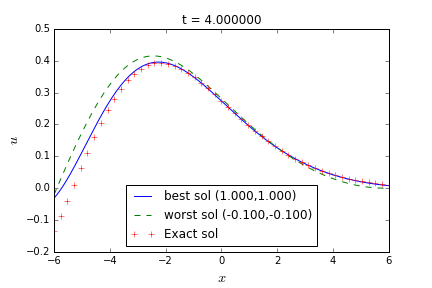
\includegraphics[scale=.5]{figures/BessefirstTestsP0Snap5.png}
\end{minipage}
\captionof{figure}{Best and worst solution compared with analytical solution, for the constant polynomial approximation \label{fig:firstTestsP0}}
\endgroup

\indent Le tableau \ref{tab:firstTestsP0} présente les dix tests qui ont donné les erreurs $e_{L2}$ les plus petites :

\sisetup{round-mode=places}
\begin{center}
\begin{tabular}{c|c|S[round-precision=4,table-number-alignment =  left]}
	\multicolumn{1}{c|}{$c_L$}  & \multicolumn{1}{c|}{$c_R$} & \multicolumn{1}{r}{$e_{L2}$} \\
	\hline
	1.0 & 1.0 & 0.0946839239675 \\
	1.0 & 10.0 & 0.097288371204 \\
	1.0 & 0.1 & 0.0983932287563 \\
	1.0 & 0.0 & 0.0992063806502 \\
	1.0 & -10.0 & 0.099359192771 \\
	1.0 & -0.1 & 0.100021589665 \\
	1.0 &  -1. & 0.10159265619 \\
	10.0 & 1.0 & 0.347003021321 \\
	10.0 & 0.1 & 0.347379492262 \\
	10.0 & 0.0 & 0.347487945035
\end{tabular}
\captionof{table}{Best results (smallest $e_{L2}$) for the constant polynomial approximation \label{tab:firstTestsP0}}
\end{center}

\indent On remarque que les résultats sont beaucoup plus sensitives au coefficient pour le bord à gauche : pour un $c_L$ fixé, l'erreur est très similaire pour tout $c_R$. Cela est une conséquence du fait que la solution de ce problème est pratiquement constante et égale à zéro aux voisinages de $x = 6$, mais présente des fortes variations dans la région proche de  $x = -6$. Le meilleur résultat, comme montre la figure \ref{fig:firstTestsP0}, est capable d'imposer ce condition dans le bord à droite, tandis que la pire solution n'en peut pas. Dans le cas du bord à gauche, malgré une erreur plus évidente, les meilleures solutions suivent approximativement bien le comportement de la solution exacte.

\subsection{Approximation des TBCs utilisant un polynôme linéaire}

\indent De façon similaire à ce qu'on a fait ci-dessus, on approxime $\frac{\lambda^2}{s}$ par $P_1(s) = ds + c$. Puis, en établissant des relations comme \eqref{eq:appP0}, les convolutions dans \eqref{eq:continuousTBC} s'écrivent :

\begin{equation*}
	\begin{aligned}
    \mathcal{L}^{-1} \left( \frac{\lambda^2}{s}\right) *  u_x(s,x)   =  & \  \mathcal{L}^{-1} \left( \frac{\lambda^2}{s} \hat{u}_x(s,x) \right) =  \mathcal{L}^{-1} \left[ (ds+c) \hat{u}_x(t,s) \right] = \\
    			 & d\mathcal{L}^{-1} \left[ \hat{u}_{xt}(t,s) \right] + c \mathcal{L}^{-1} \left[ \hat{u}_{x}(t,s) \right] = \\
    			 &   du_{xt}(x,t) + du_x(0,x)\delta (t) + cu_x(x,t) \\
    \mathcal{L}^{-1} \left( \frac{\lambda}{s} \right) * u_{xx}(s,x)  = & \   \mathcal{L}^{-1} \left( \frac{\lambda}{s} \hat{u}_{xx}(s,x) \right) =  \mathcal{L}^{-1} \left[ -(ds+c)^2 \hat{u}_{xx}(t,s) \right] =\\
    			&  -d^2u_{xxtt}(x,t) - d^2\delta_t(t) u_xx(0,x) - d^2 \delta(t)u_{xxt}(0,x)  + \\ 
    			& - 2dcu_{xxt}(x,t) -  2dcu_xx(0,x)\delta (t) - c^2u_{xx}(x,t) \\
     \mathcal{L}^{-1} \left( \frac{1}{\lambda^2} \right) * u_{xx}(s,x)  = & \  \mathcal{L}^{-1} \left( \frac{1}{\lambda^2} \hat{u}_{xx}(s,x) \right) = \mathcal{L}^{-1} \left[ (ds+c)^2 \hat{u}_{xx}(t,s) \right] = \\
    			& d^2u_{xxtt}(x,t) + d^2\delta_t(t) u_xx(0,x) + d^2 \delta(t)u_{xxt}(0,x)  + \\
    			& 2dcu_{xxt}(x,t) +  2dcu_xx(0,x)\delta (t) + c^2u_{xx}(x,t) \\
     \mathcal{L}^{-1} \left( \frac{1}{\lambda} \right) u_{xx}(s,x) = & \  \mathcal{L}^{-1} \left( \frac{1}{\lambda} \hat{u}_{xx}(s,x) \right) = \mathcal{L}^{-1} \left[ -(ds+c) \hat{u}_{xx}(t,s) \right] = \\
    			& -du_{xxt}(x,t) - du_{xx}(0,x)\delta (t) - cu_{xx}(x,t)
\end{aligned}
\end{equation*}

\indent En utilisant des différences finies pour les dérivées en temps, et en considérant que la solution initiale est nulle sur les bords (ce qui est le cas de l'exemple testé ici), on obtient les TBC approximées discrètes : 

\begin{equation*}
\label{eq:appDiscTBCP1}
	\begin{gathered}
    u_0^{n+1} - \left( \frac{d_L}{\Delta t} + c_L \right) \left( \frac{u_1^{n+1} - u_0^{n+1}}{\Delta x}\right) +   \left( \frac{d_L^2}{\Delta t^2} + \frac{2d_Lc_L}{\Delta t} + c_L^2  \right) \left(  \frac{u_0^{n+1} - 2u_1^{n+1} + u_2^{n+1}}{\Delta x^2} \right)  = \\
        -\frac{d_L}{\Delta t}\left( \frac{u_1^{n} - u_0^{n}}{\Delta x}\right) +  \left( 2\frac{d_L^2}{\Delta t^2} + \frac{2d_Lc_L}{\Delta t}\right) \left(  \frac{u_0^{n} - 2u_1^n + u_2^{n}}{\Delta x^2} \right)    -  \frac{d_L^2}{\Delta t^2} \left(  \frac{u_0^{n-1} - 2u_1^{n-1} + u_2^{n-1}}{\Delta x^2} \right)
   \end{gathered}
\end{equation*} 

\begin{equation*}
	\begin{aligned}
    u_N^{n+1} - \left( \frac{d_R^2}{\Delta t^2} + \frac{2d_Rc_R}{\Delta t} + c_R^2  \right) \left(  \frac{u_{N}^{n+1} - 2u_{N-1}^{n+1} + u_{N-2}^{n+1}}{\Delta x^2} \right) = \\
     -\left( 2\frac{d_R^2}{\Delta t^2} + \frac{2d_Rc_R}{\Delta t}\right) \left(  \frac{u_N^{n} - 2u_{N-1}^n + u_{N-2}^{n}}{\Delta x^2} \right) + \frac{d_R^2}{\Delta t^2} \left(  \frac{u_N^{n-1} - 2u_{N-1}^{n-1} + u_{N-2}^{n-1}}{\Delta x^2} \right)
    \end{aligned}
\end{equation*} 
   
\begin{equation*}
	\begin{aligned}	
    \frac{u_N^{n+1} - u_{N-1}^{n+1}}{\Delta x} + \left( \frac{d_R}{\Delta t} + c_R \right) \left( \frac{u_N^{n+1} -2 u_{N-1}^{n+1} + u_{N-2}^{n+1}}{\Delta x^2}\right) =      \frac{d_R}{\Delta t}\left( \frac{u_{N}^{n} - 2u_{N-1}^{n} + u_{N-2}^n}{\Delta x^2}\right)
    \end{aligned}
\end{equation*}

\subsubsection{Tests de validation de l'approximation}

\indent On répète les tests faites pour l'approximation avec $P_0$, en faisant varier les coefficients $c_L$ et $c_R$ parmi les valeurs dans $\{-10,-1,-0.1,0,0.1,1,10\}$. Afin d'éviter un calcul trop longue, et aussi en utilisant la remarque fait ci-dessus concernant la faible influence des coefficients du bord à droite sur les résultats, tous les tests seront faits avec $c_R = c_L$ et $d_R = d_L$.

\indent Les dix meilleurs résultats sont présentés dans le tableau \ref{tab:firstTestsP1}. On observe que le meilleur résultat est celui avec $d_L = d_R = 0$ et $c_L = c_R = 1. $, ce qui correspond au meilleur résultat parmi les approximations utilisant des polynômes constants.


%	 \sisetup{round-mode=places}
%\begin{center}
%\begin{tabular}{c|c|S[round-precision=4,table-number-alignment =  left]}
%	\multicolumn{1}{c|}{$d_L = d_R$}  & \multicolumn{1}{c|}{$c_L = c_R$} & \multicolumn{1}{r}{$e_{L2}$} \\
%	\hline
%	0. & 1.0 & 0.0946839239675 \\
%	0.1 & 1.0 & 0.12341195 \\
%	1.0 & 1.0 & 0.20031603 \\
%	10.0 & 0.1 & 0.22037249 \\
%	-10.0 & 0.1 & 0.23984486 \\
%	10.0 & 1.0 & 0.27161158 \\
%	-10.0 &  0.0 & 0.24800816\\
%	-10.0 & 1.0 & 0.30039637 \\
%	10.0 & 0.0 & 0.27213611 \\
%	0.0 & 0.1 & 0.36740764
%\end{tabular}
%\captionof{table}{Meilleurs résultas (les erreurs $e_{L2}$ les plus petites) pour l'approximation avec le polynôme linéaire \label{tab:firstTestsP1}}
%\end{center}

	 \sisetup{round-mode=places}
\begin{center}
\begin{tabular}{c|c|S[round-precision=4,table-number-alignment =  left]}
	\multicolumn{1}{c|}{$d_L = d_R$}  & \multicolumn{1}{c|}{$c_L = c_R$} & \multicolumn{1}{r}{$e_{L2}$} \\
	\hline
	0. & 1.0 & 0.10754381 \\
	0.1 & 1.0 & 0.14050496 \\
	1.0 & 1.0 & 0.19200976 \\
	10.0 & 0.1 & 0.22789348 \\
	-10.0 & 0.1 & 0.37713227 \\
	10.0 & 1.0 & 0.27161158 \\
	-10.0 &  0.0 & 0.24800816\\
	-10.0 & 1.0 & 0.30039637 \\
	10.0 & 0.0 & 0.27213611 \\
	0.0 & 0.1 & 0.36740764
\end{tabular}
\captionof{table}{Meilleurs résultas (les erreurs $e_{L2}$ les plus petites) pour l'approximation avec le polynôme linéaire \label{tab:firstTestsP1}}
\end{center}

\subsection{Conclusion partiale}

\indent Il faut être claire que notre approximation ne fournit pas des meilleures TBCs que celles proposées par \cite{besse2015} (et cela n'est pas non plus l' objectif du travail développé ici, comme il a été discuté dans la introduction de ce rapport). En fait, \cite{besse2015} dérive des TBCs pour deux schémas discrets, et le pire résultat parmi eux, en utilisant les mêmes $\Delta t$ et $\Delta x$ utilisés ici, présente une erreur $e_{L2} \approx 0.005$ pour $t = 4$, tandis que notre mieux résultat fournit $e_{L2} \approx 0.1$ pour le même instant. Néanmoins, en considérant qu'on souhaite appliquer les TBCs à une Méthode de Décomposition de Domaine, on voudra minimiser l'erreur due à les conditions limites à l'interface, mais pas l'erreur liée aux conditions aux limites extérieures.

\indent Cependant, enc considérant les résultats présentés jusqu'ici, on peut dire que les conditions aux limites proposées simulent relativement bien des TBCs, avec une implémentation assez simple, en comparaison avec celles proposées par \cite{besse2015} (qui demandent par exemple le calcul de $\mathcal{Z}$-transformées, dans le rôle de versions discrètes des Transformées de Laplace). Par ailleurs, on remarque que l'approximation qu'on a fait avec le polynôme linéaire, malgré l'augmentation de la complexité du schéma (où il faut garder la solution des itérations précédentes), ne fournit pas des meilleures résultats par rapport au cas du polynôme constant.

\indent Ainsi, dans la suite, on va utiliser toujours l'approximation avec $P_0$. On notera les TBCs correspondantes avec les opérateurs $\theta_i^c, \ i=1,2,3$, définis dans \eqref{eq:appTBCP0}.

\begin{equation*}
    \begin{gathered}
        \Theta_1^{c_L}(u,x) = u(t,x) - c_L u_x(t,x)  + c_L^2  u_{xx}(t,x) \\
        \Theta_2^{c_R}(u,x) =  u(t,x) - c_R^2    u_{xx}(t,x)\\
        \Theta_3^{c_R} (u,x)= u_x(t,x) + c_R u_{xx}(t,x) 
    \end{gathered}
\end{equation*}